\newpage
\hypertarget{allCards tex}{}
\subsection{AllOtherCardsRule}
\texHeader

\begin{itemize}

\item[$\blacktriangleright$] Right click on the \texttt{rules} folder again and create \texttt{AllOtherCardsRule}. Complete the rule until your file resembles
Fig.~\ref{fig:eclipse_allOtherCardsRule}.

\vspace{0.5cm}

\begin{figure}[htbp]
\begin{center}
  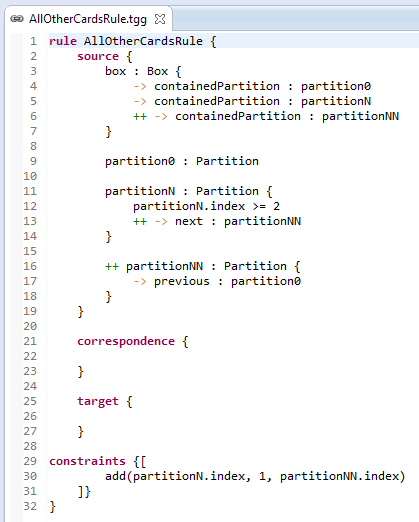
\includegraphics[width=0.7\textwidth]{eclipse_allOtherCardsRule}
  \caption{All Other Cards Rule Complete}
  \label{fig:eclipse_allOtherCardsRule}
\end{center}
\end{figure}

\item[$\blacktriangleright$] You'll notice that \texttt{box} and \texttt{partition0} have been established as `black' objects -- this rule may only be evaluated
when these objects are already known (and simply need to be adjusted), so we can use their values from the context of the transformation.

\vspace{0.5cm}

\item[$\blacktriangleright$] A second partition, \texttt{partitionN}, has also been established fromt he context. It represents the \texttt{n}th or last
partition in a \texttt{box} (with an index of 2 or higher), whose \texttt{next} reference will be updated in order to provide an access
link to the newest element, \texttt{partitionNN}.

\newpage

\item[$\blacktriangleright$] Given that the \texttt{add(a,b,c)} syntax is \texttt{a+b=c}, the sole constraint of this rule sets the \texttt{index} of the
\texttt{n+1}th partition so that the \texttt{partition}s are still listed in order.

\vspace{0.5cm}

\item[$\blacktriangleright$] That's it! Save and build your package explorer, then run the TGG again with the `extra' \texttt{partition} to confirm it worked!
You are now free to add as many \texttt{partition}s and \texttt{card}s to \texttt{source.xmi} -- the transformation is now able to handle them all.

\vspace{0.5cm}

\item[$\blacktriangleright$] Be sure to check out how this rule is implemented in eMoflon's visual specification in Fig.~\ref{fig:ea_allOtherCardsRule} from the
previous section.

\end{itemize}
